% !TeX root = paper.tex


\chapter{システムについて}\label{system}
%\section{この章で書くこと}
%\begin{itemize}
%	\item 識別,分類とは
%	\item 現存するサービスでできること
%	\item 概要図
%	\item モデルについて
%	\item サーバ関連について
	%\item もしかしたらあんまり書くことないかも
%\end{itemize}
\section{分類と識別とは}
%参考文献:https://business.ntt-east.co.jp/content/cloudsolution/column-391.html
分類はデータやオブジェクトを異なるクラスやカテゴリに分けるプロセスを指す.画像の分類とは,画像が特定のカテゴリやクラスに属するかどうかを判別する作業である.例えば,画像に写っているのが猫か犬かのクラスに分けることである.

識別とは画像のどこに何が写っているのかを判別するプロセスを指す.1枚の画像に複数の物体が存在する場合も識別はできる.動画に写っている電車の車両タイプも判別することができる.



\section{現存するサービス}
現在車両タイプを調べるためには,Googleレンズを利用することや図鑑と見比べることの2つが挙げられる.
Google レンズとは画像の分類を行うアプリである.単に分類結果が表示されるのではなく,分類したいオブジェクトが映っているウェブサイト一覧が表示されるものである.表示されたウェブサイトを適当に選び自分が知りたい結果をウェブサイトの中から探し出す必要がある.また,一枚の画像に複数のオブジェクトが存在している場合は正しい結果が得られない.


\section{YOLO}
YOLOとはYou Only Look Onceの略で,人間のように一目見るだけで物体検出ができることを指している\cite{YOLO}.データセットを作成し学習させることで,任意の物体のみ検出させることが可能である.
YOLOv8はYOLOシリーズの最新バージョンであり,ディープラーニングとコンピュータビジョンの最先端の進歩に基づいており,速度と精度の麺で比類のない性能を提供している.
%https://docs.ultralytics.com/ja/ 参照
本プロジェクトでは,YOLOv8を用いて電車の車両タイプを識別,分類する2つのモデルを開発する.

====ここから田村=====

\section{システム概要図}
本プロジェクトで開発するシステム概要を図\ref{FIG}に示す.システムは車両判別部とUIに分けられる.

\begin{figure}
	\centering
	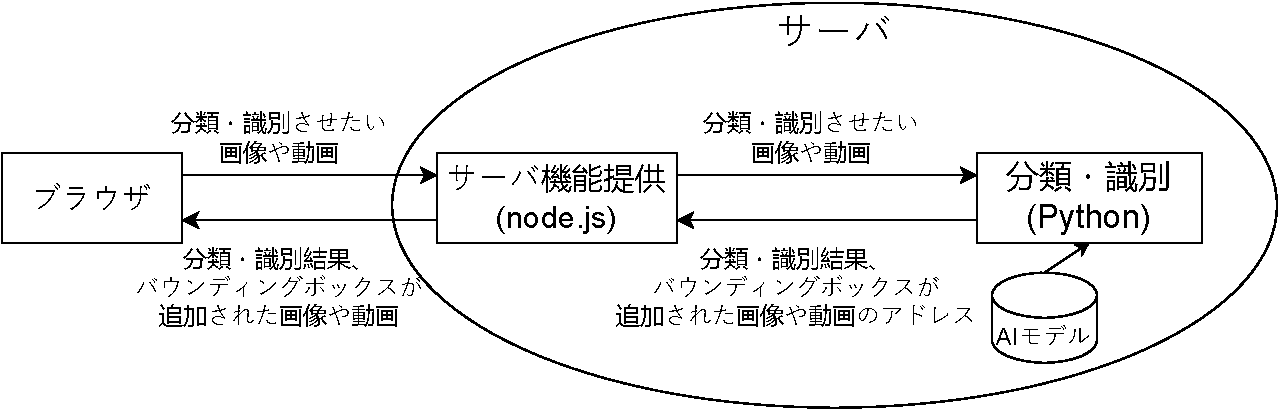
\includegraphics [width=\linewidth]{chap2/fig/sys_gaiyou6.pdf}
	\caption{システム概要図}
	\label{FIG}
\end{figure}

\section{動作環境,開発環境}
動作環境,開発環境
\section{システムの機能}
分類,識別,
\section{動作確認と現状}
動作確認

